\section{Problem definition}

\subsection{Informative path}

\begin{frame}{Coverage model}{Informative path}

\begin{itemize}
\item Maximum coverage problem
\item Information gain - entropy 
\end{itemize}

\begin{figure}
\centering
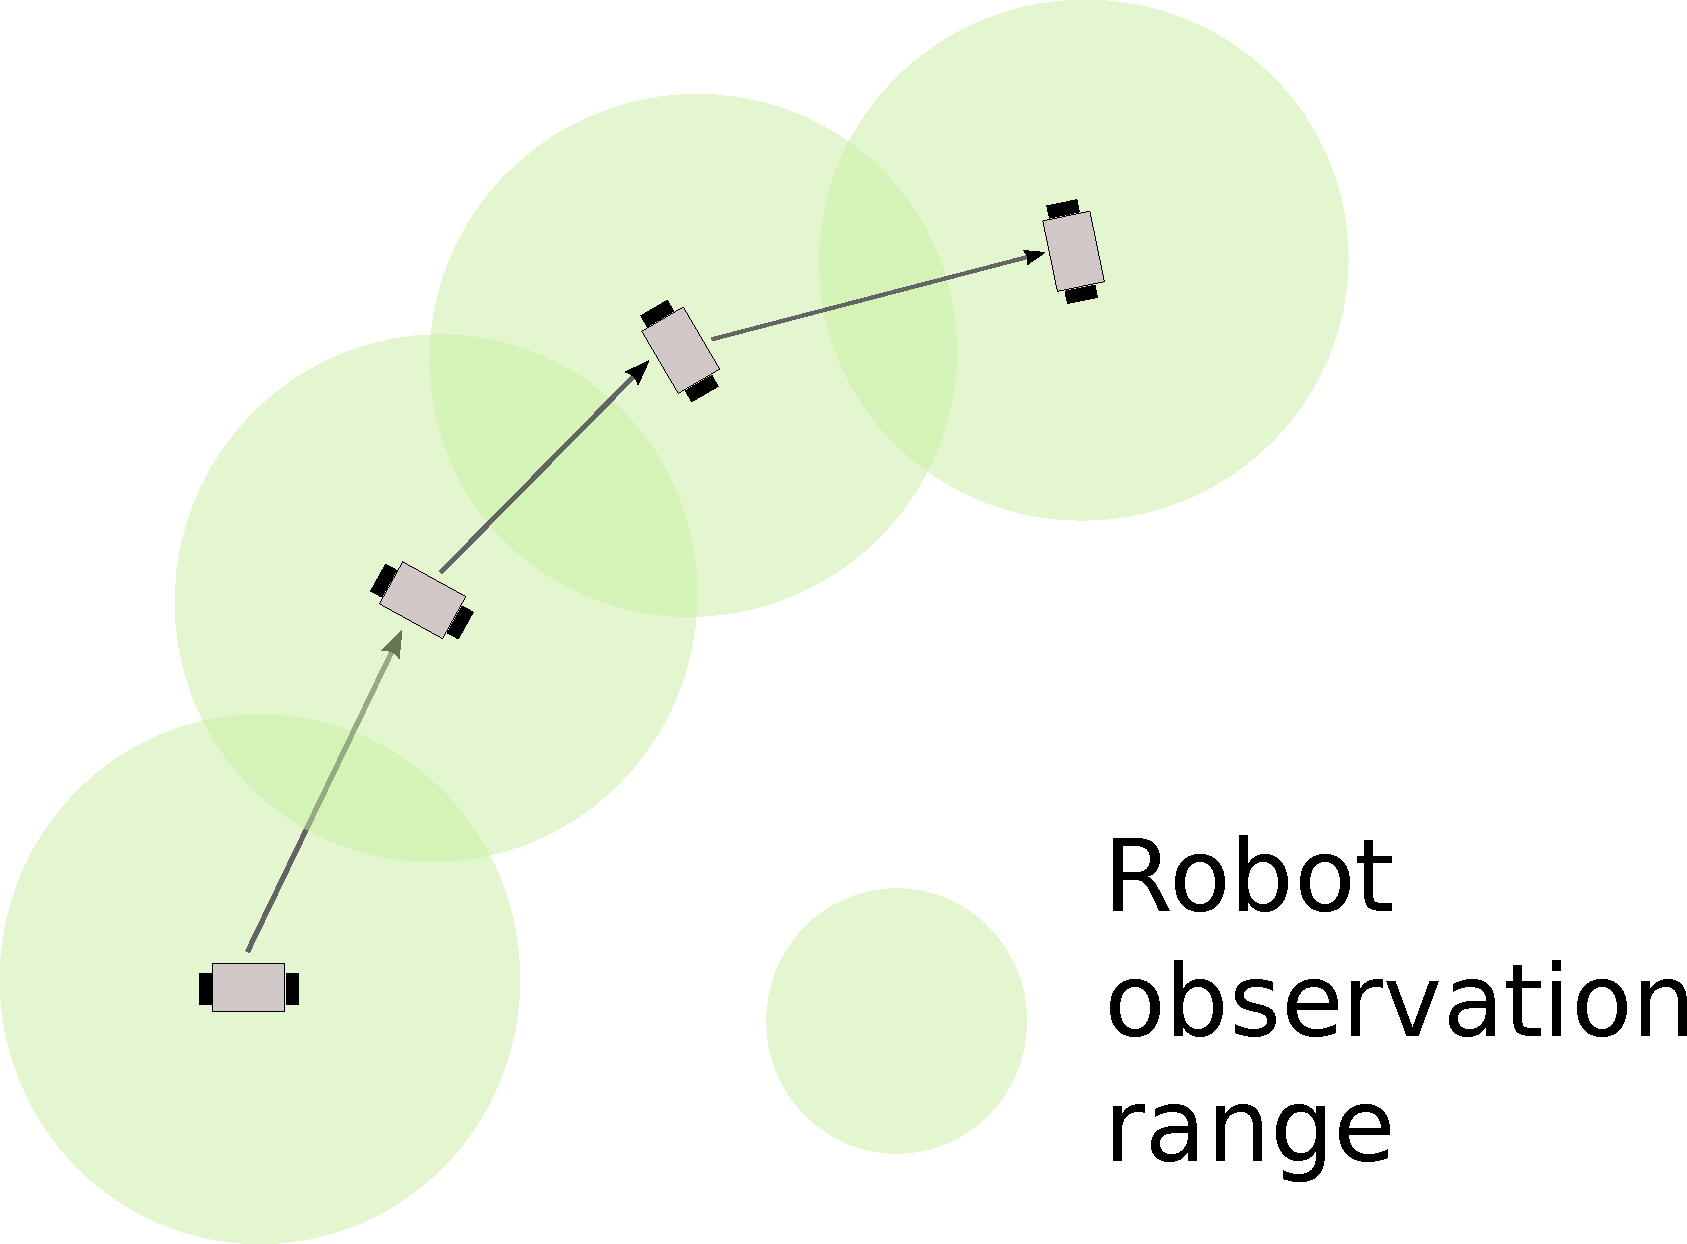
\includegraphics[width = 0.6\textwidth]{./figure/robotObservation}
%\caption{A coverage model.}
\end{figure}

\end{frame}

\begin{frame}{Submodularity}{Informative path}

\begin{columns}

\column{0.45\textwidth}

\begin{figure}
\centering
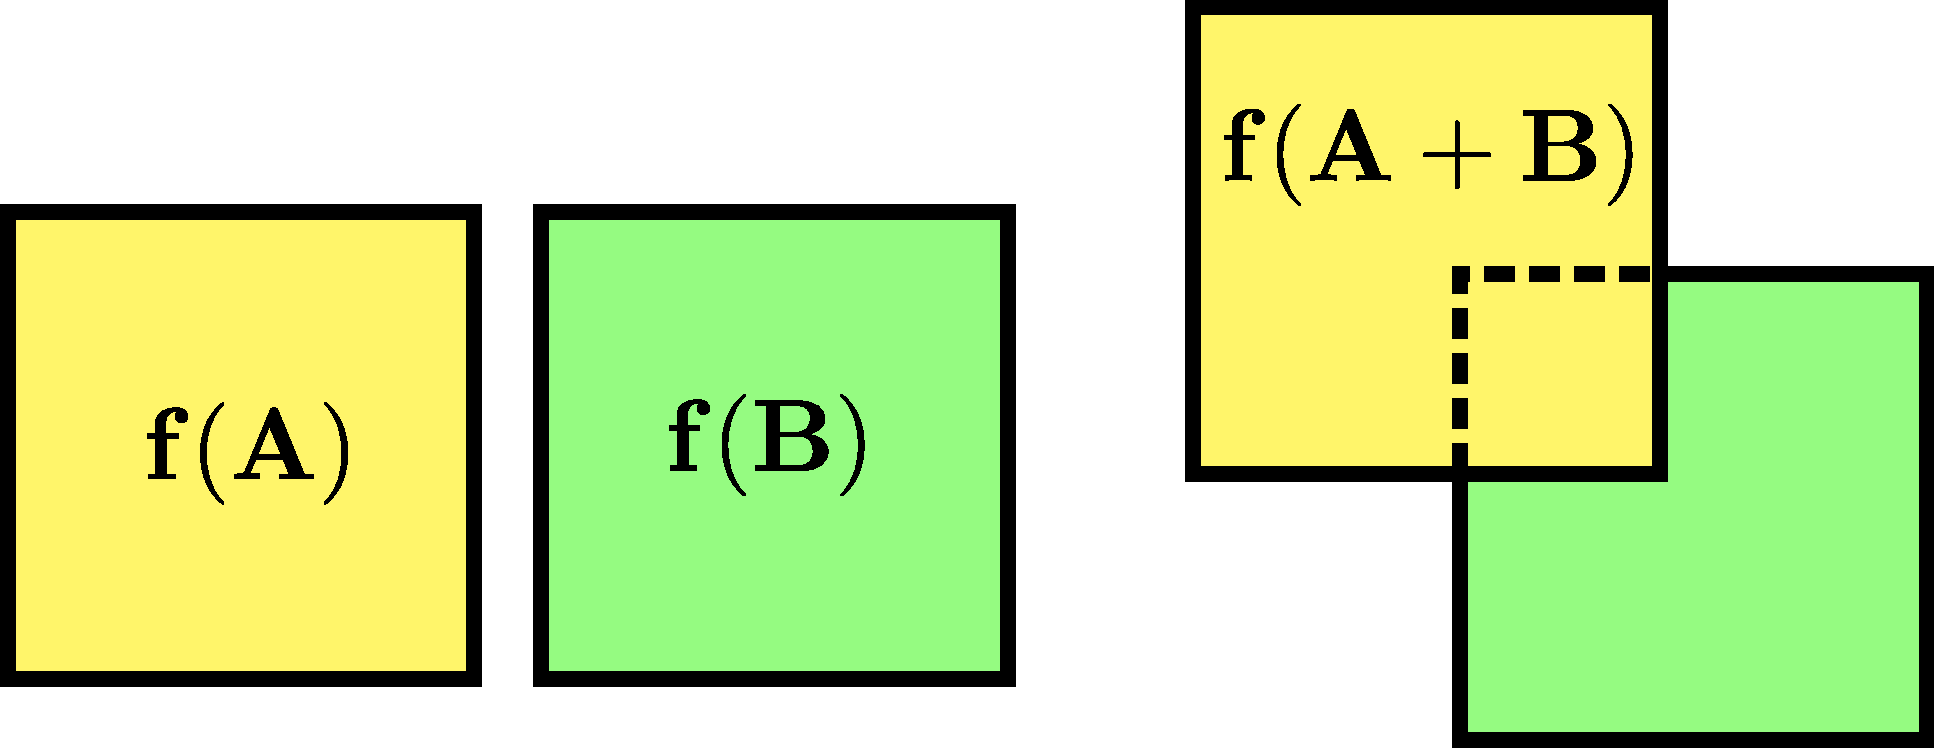
\includegraphics[width = \textwidth]{./figure/submodular}
%\caption{A coverage model.}
\end{figure}

\begin{equation}
\nonumber
f(A) + f(B) \geq f(A+B)
\end{equation}

\column{0.1\textwidth}

\column{0.45\textwidth}

Information
\begin{itemize}
\item search space $ S $
\item the observation of a robot $ \mathbf{O}^{X} $ 
\item the observation of a human $ \mathbf{O}^{Y} $

\bigskip
\bigskip

$ f( \mathbf{S}, \mathbf{O}^{X} ) + f( \mathbf{S}, \mathbf{O}^{Y^{h}} ) \geq f( \mathbf{S}, \mathbf{O}^{X},  \mathbf{O}^{Y^{h}} ) $ 
\end{itemize}

\end{columns}

\end{frame}

\begin{frame}{Submodular orienteering}{Informative path}

\begin{block}{Conditional mutual information}
$ I(\mathbf{S}; \mathbf{O}^{X} \mid \mathbf{O}^{Y^{h}}) = H(\mathbf{S} \mid \mathbf{O}^{Y^{h}}) - H(\mathbf{S} \mid \mathbf{O}^{X},\mathbf{O}^{Y^{h}}) $
\end{block} 

\bigskip

\begin{itemize}
\item Entropy reduction
\item Submodularity
\item Chain rule \\
$ I(\mathbf{S}; \mathbf{O}^{X} \mid \mathbf{O}^{Y^{h}}) = \sum_{t=1}^{T} I(O^{X}_{t} ; \mathbf{S} \mid O^{X}_{1} , \cdots , O^{X}_{t-1}, \mathbf{O}^{Y^{h}}) $
\end{itemize}

\end{frame}

\subsection{Human constraint}

\begin{frame}{Team role}{Human constraint}

\begin{figure}
\centering
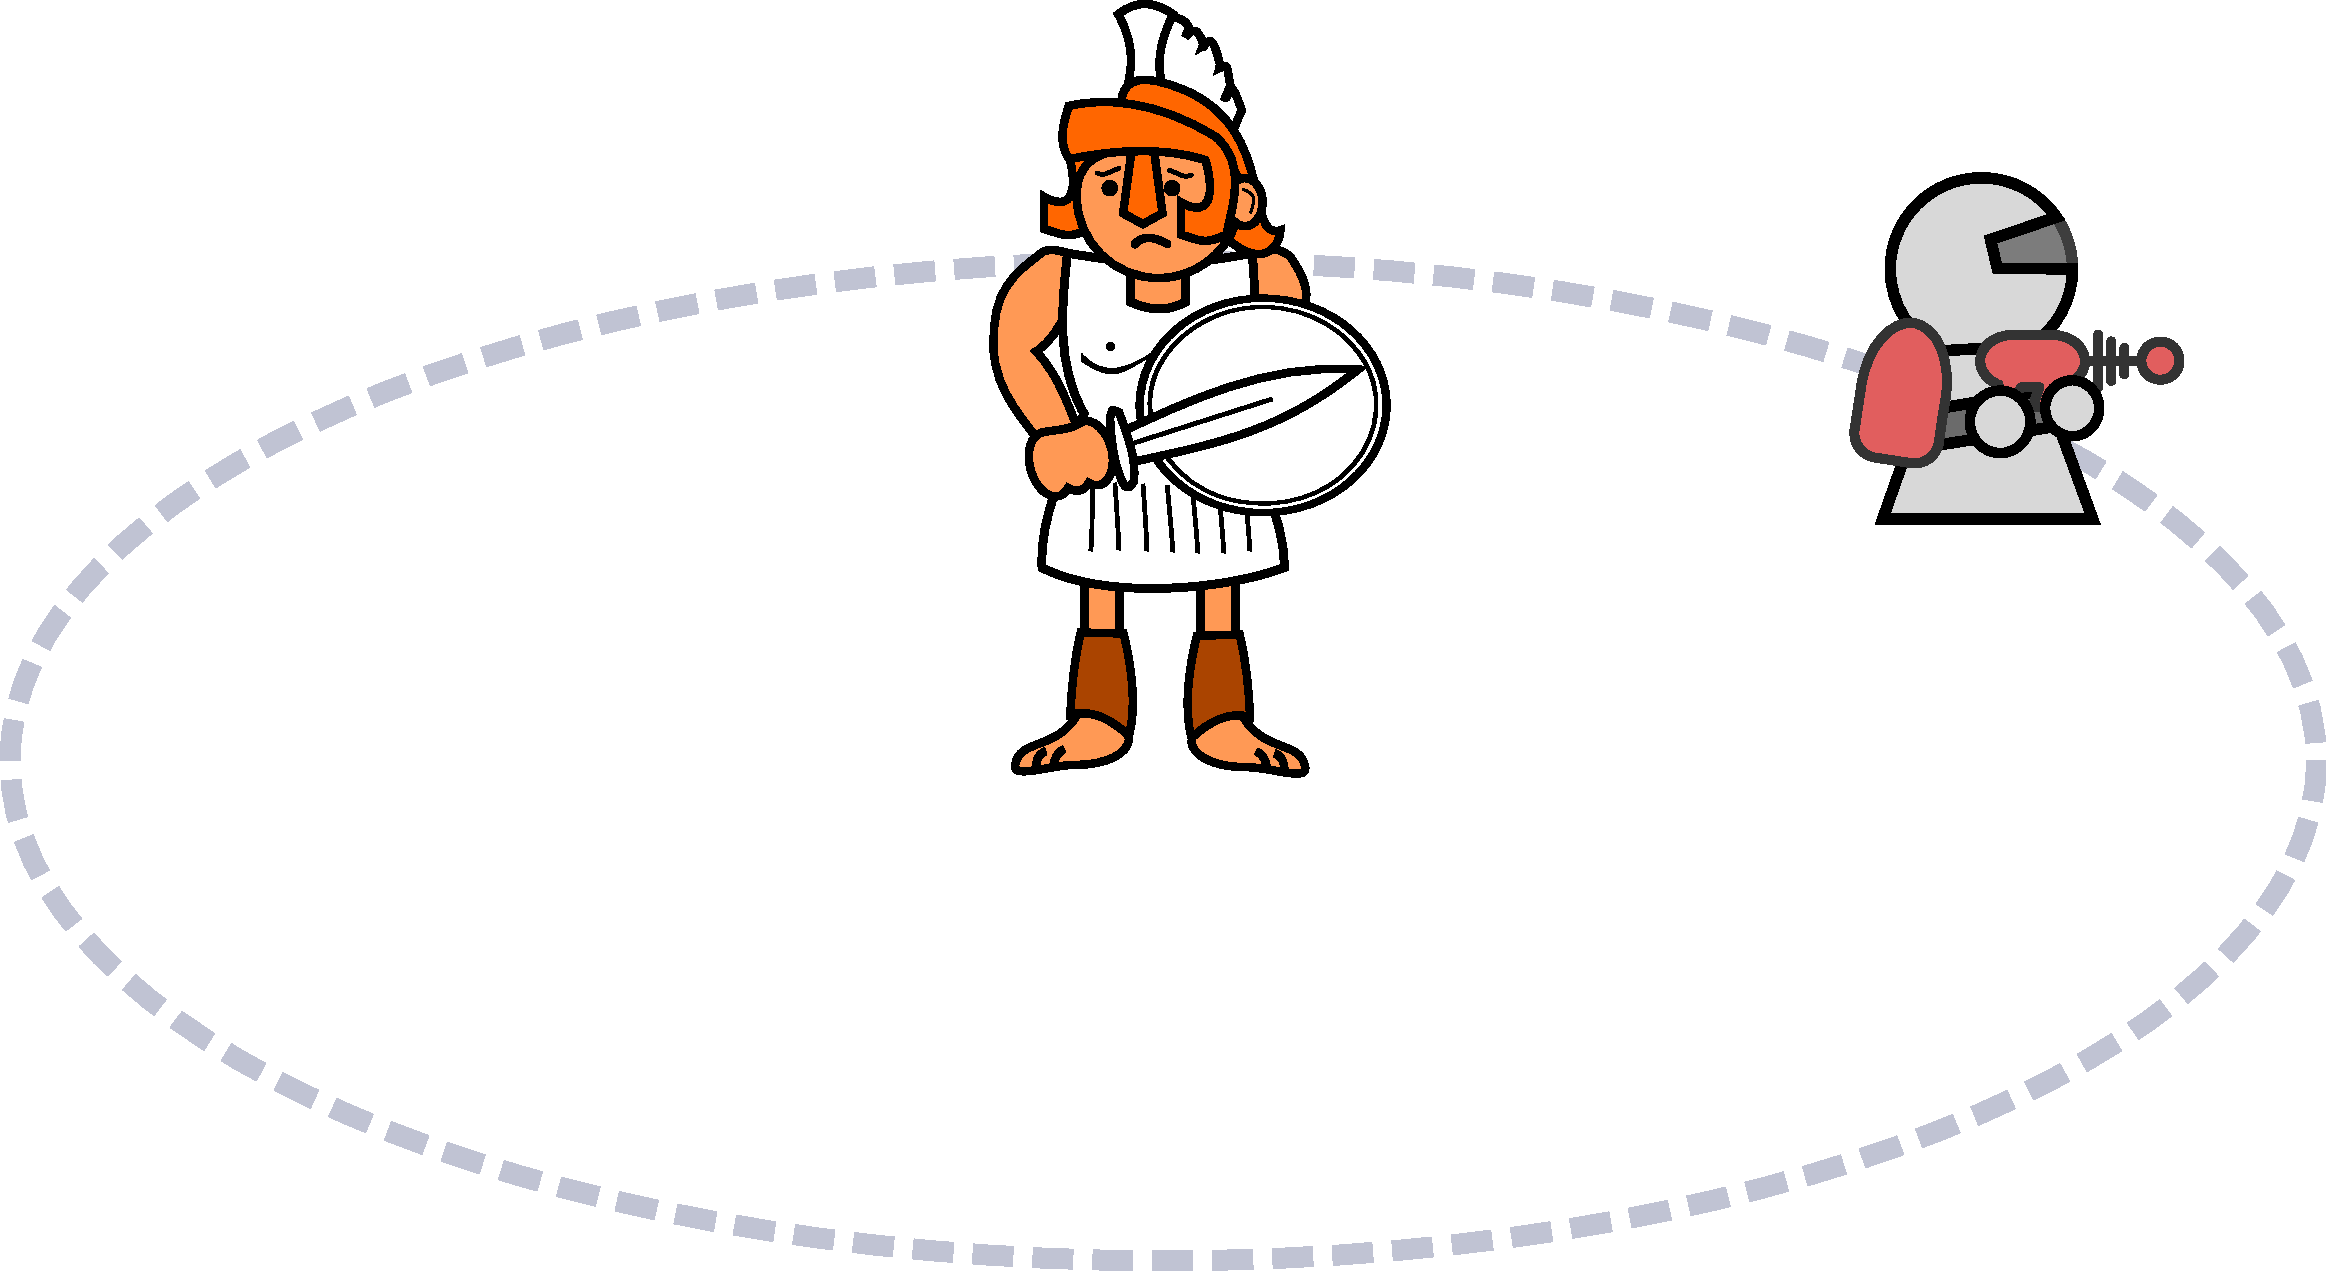
\includegraphics[width = 0.7\textwidth]{./figure/human_robot_interaction}
\end{figure}

\begin{itemize}
\item cooperative observation
\item assistance and protection
\end{itemize}

\end{frame}

\begin{frame}{Neighboring function}{Human constraint}

\begin{columns}
\column{.6\linewidth}
\begin{minipage}[c]{\linewidth}
\begin{figure}
\centering
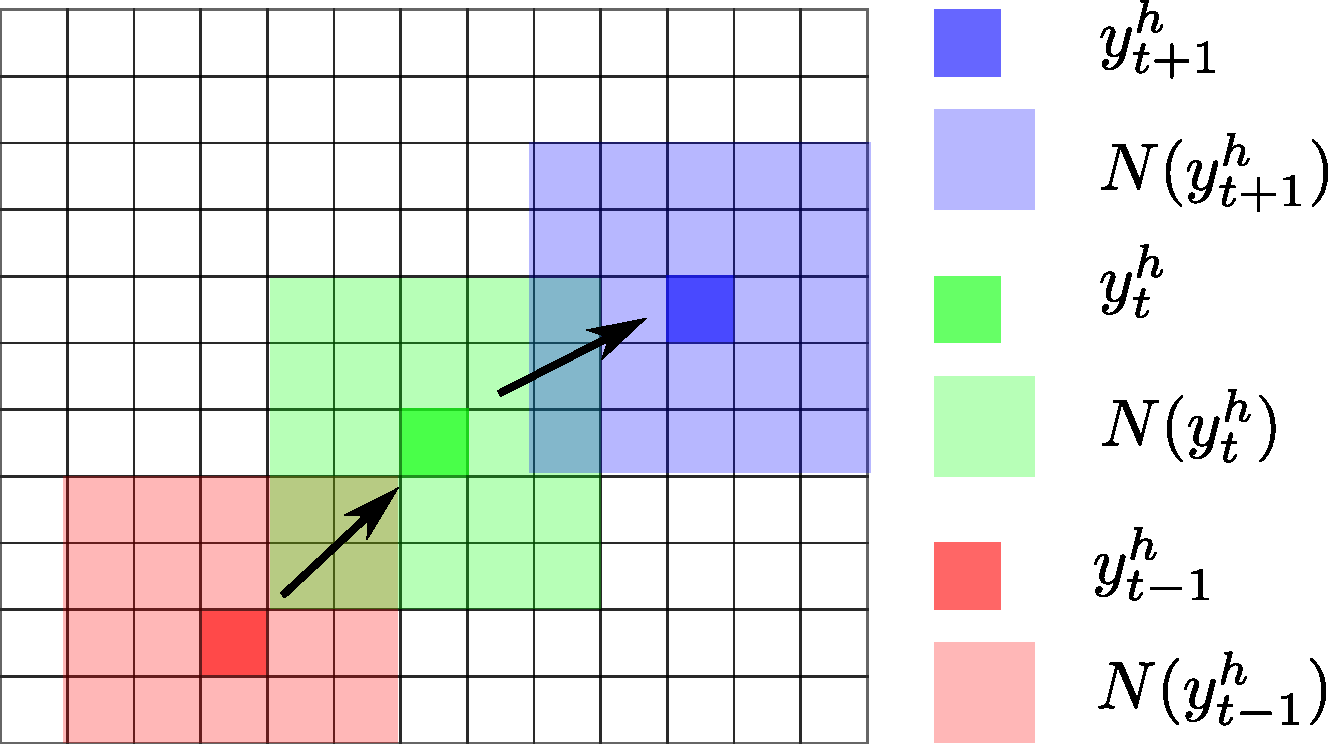
\includegraphics[width = \textwidth]{./figure/humanConstraint}
%\caption{An example of human constraint.}
\end{figure}
\end{minipage}

\column{.4\linewidth}
\begin{minipage}[c]{\linewidth}
\begin{itemize}
\item { human path $ \{ y^{h}_{1} \cdots y^{h}_{T} \} $ }
\item { neighboring function $ N( y^{h}_{t} ) $ }
\end{itemize}
\end{minipage}
\end{columns}

\end{frame}

\subsection{The optimization model}

\begin{frame}{Problem abstraction}{The optimization model}

\begin{figure}
\centering
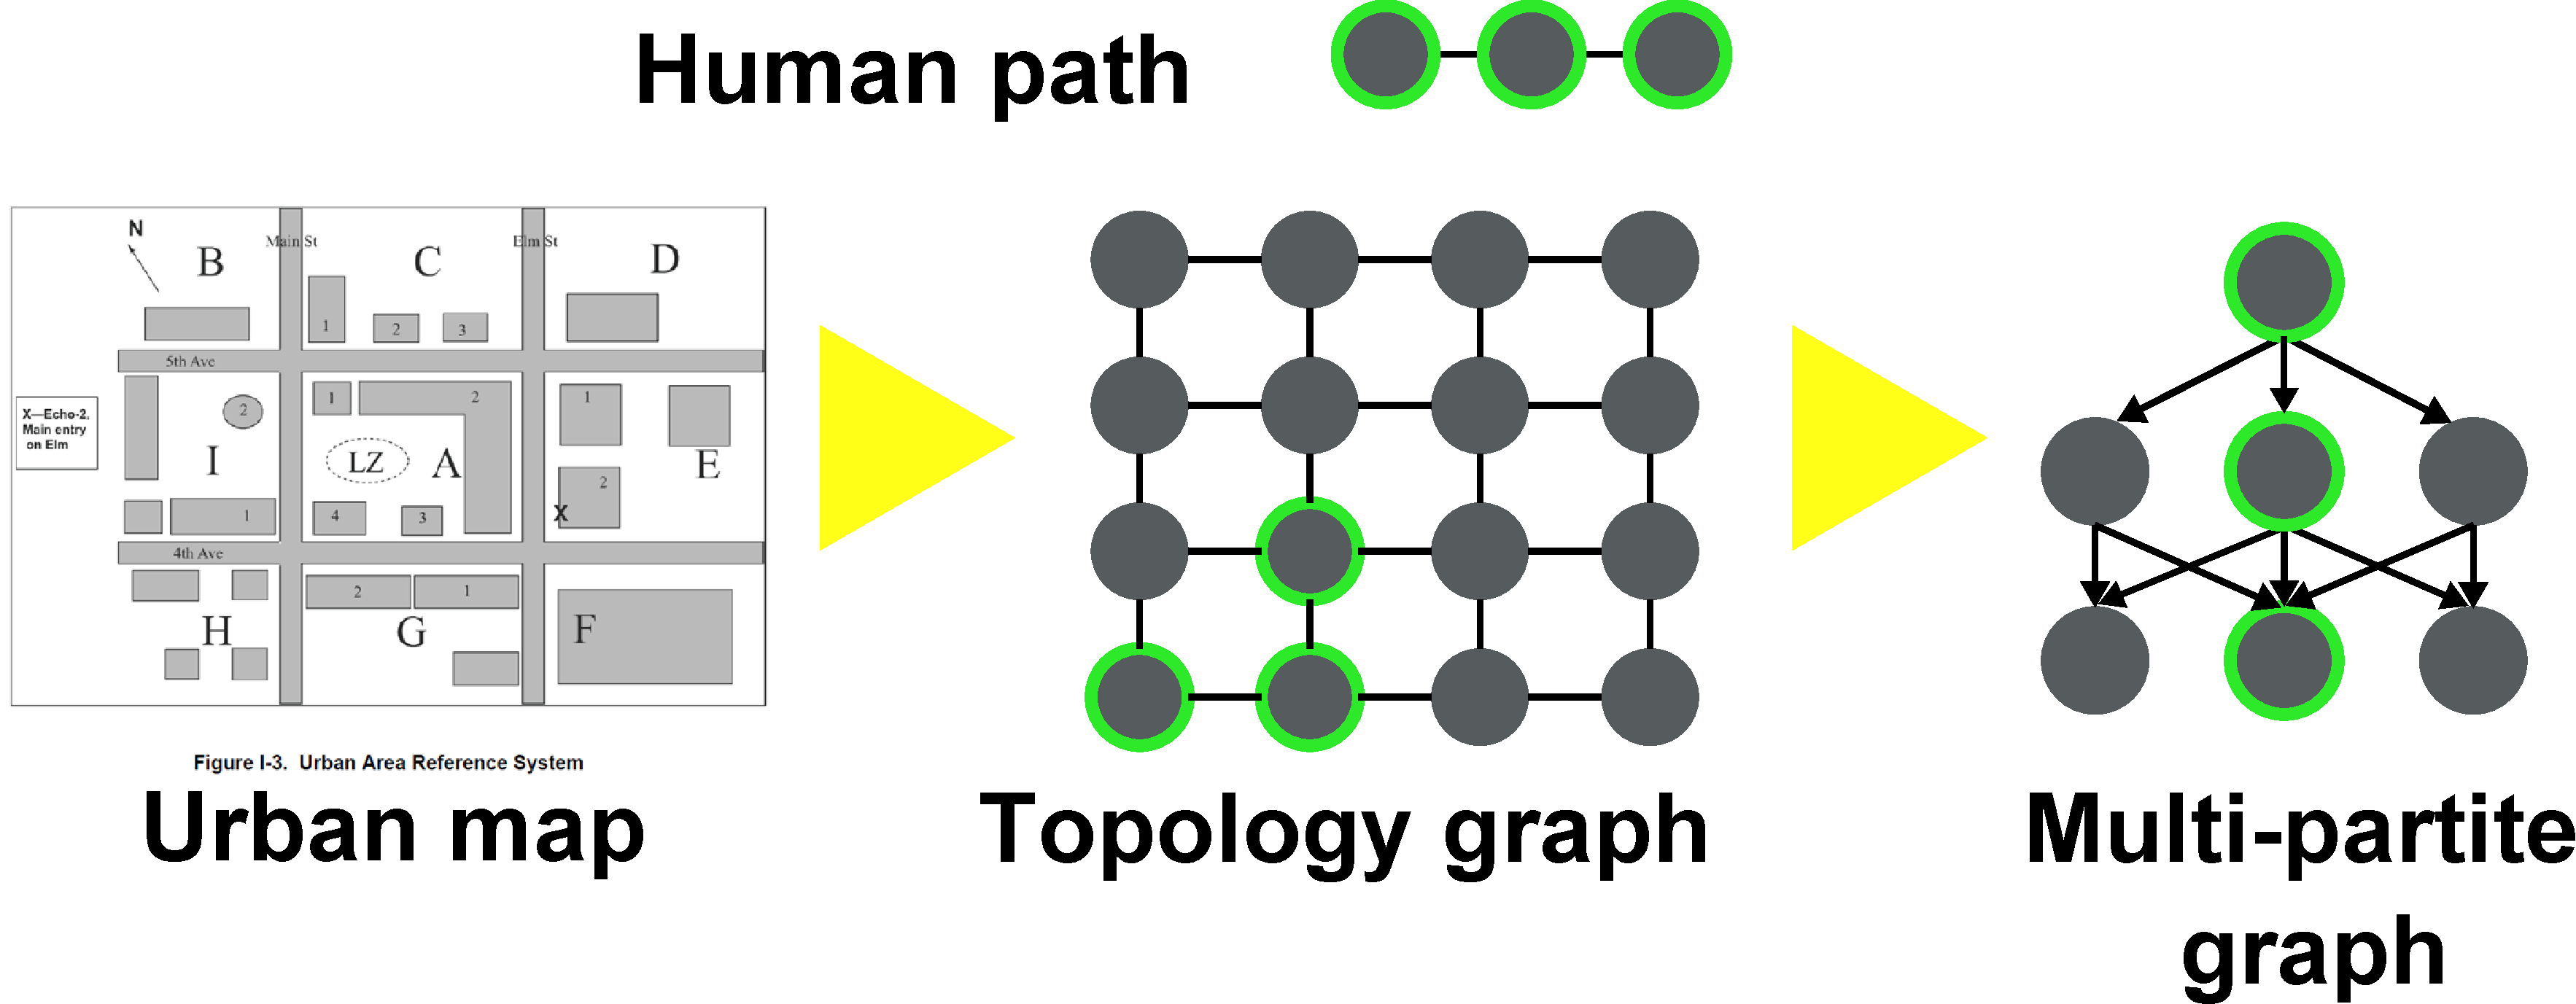
\includegraphics[width = 0.9\textwidth]{./figure/layers}
%\caption{A layered problem processing.}
\end{figure}

\end{frame}

\begin{frame}{The multi-partite graph}{The optimization model}

\begin{columns}

\column{.6\textwidth}
\begin{minipage}[c]{\linewidth}
\begin{figure}
\centering
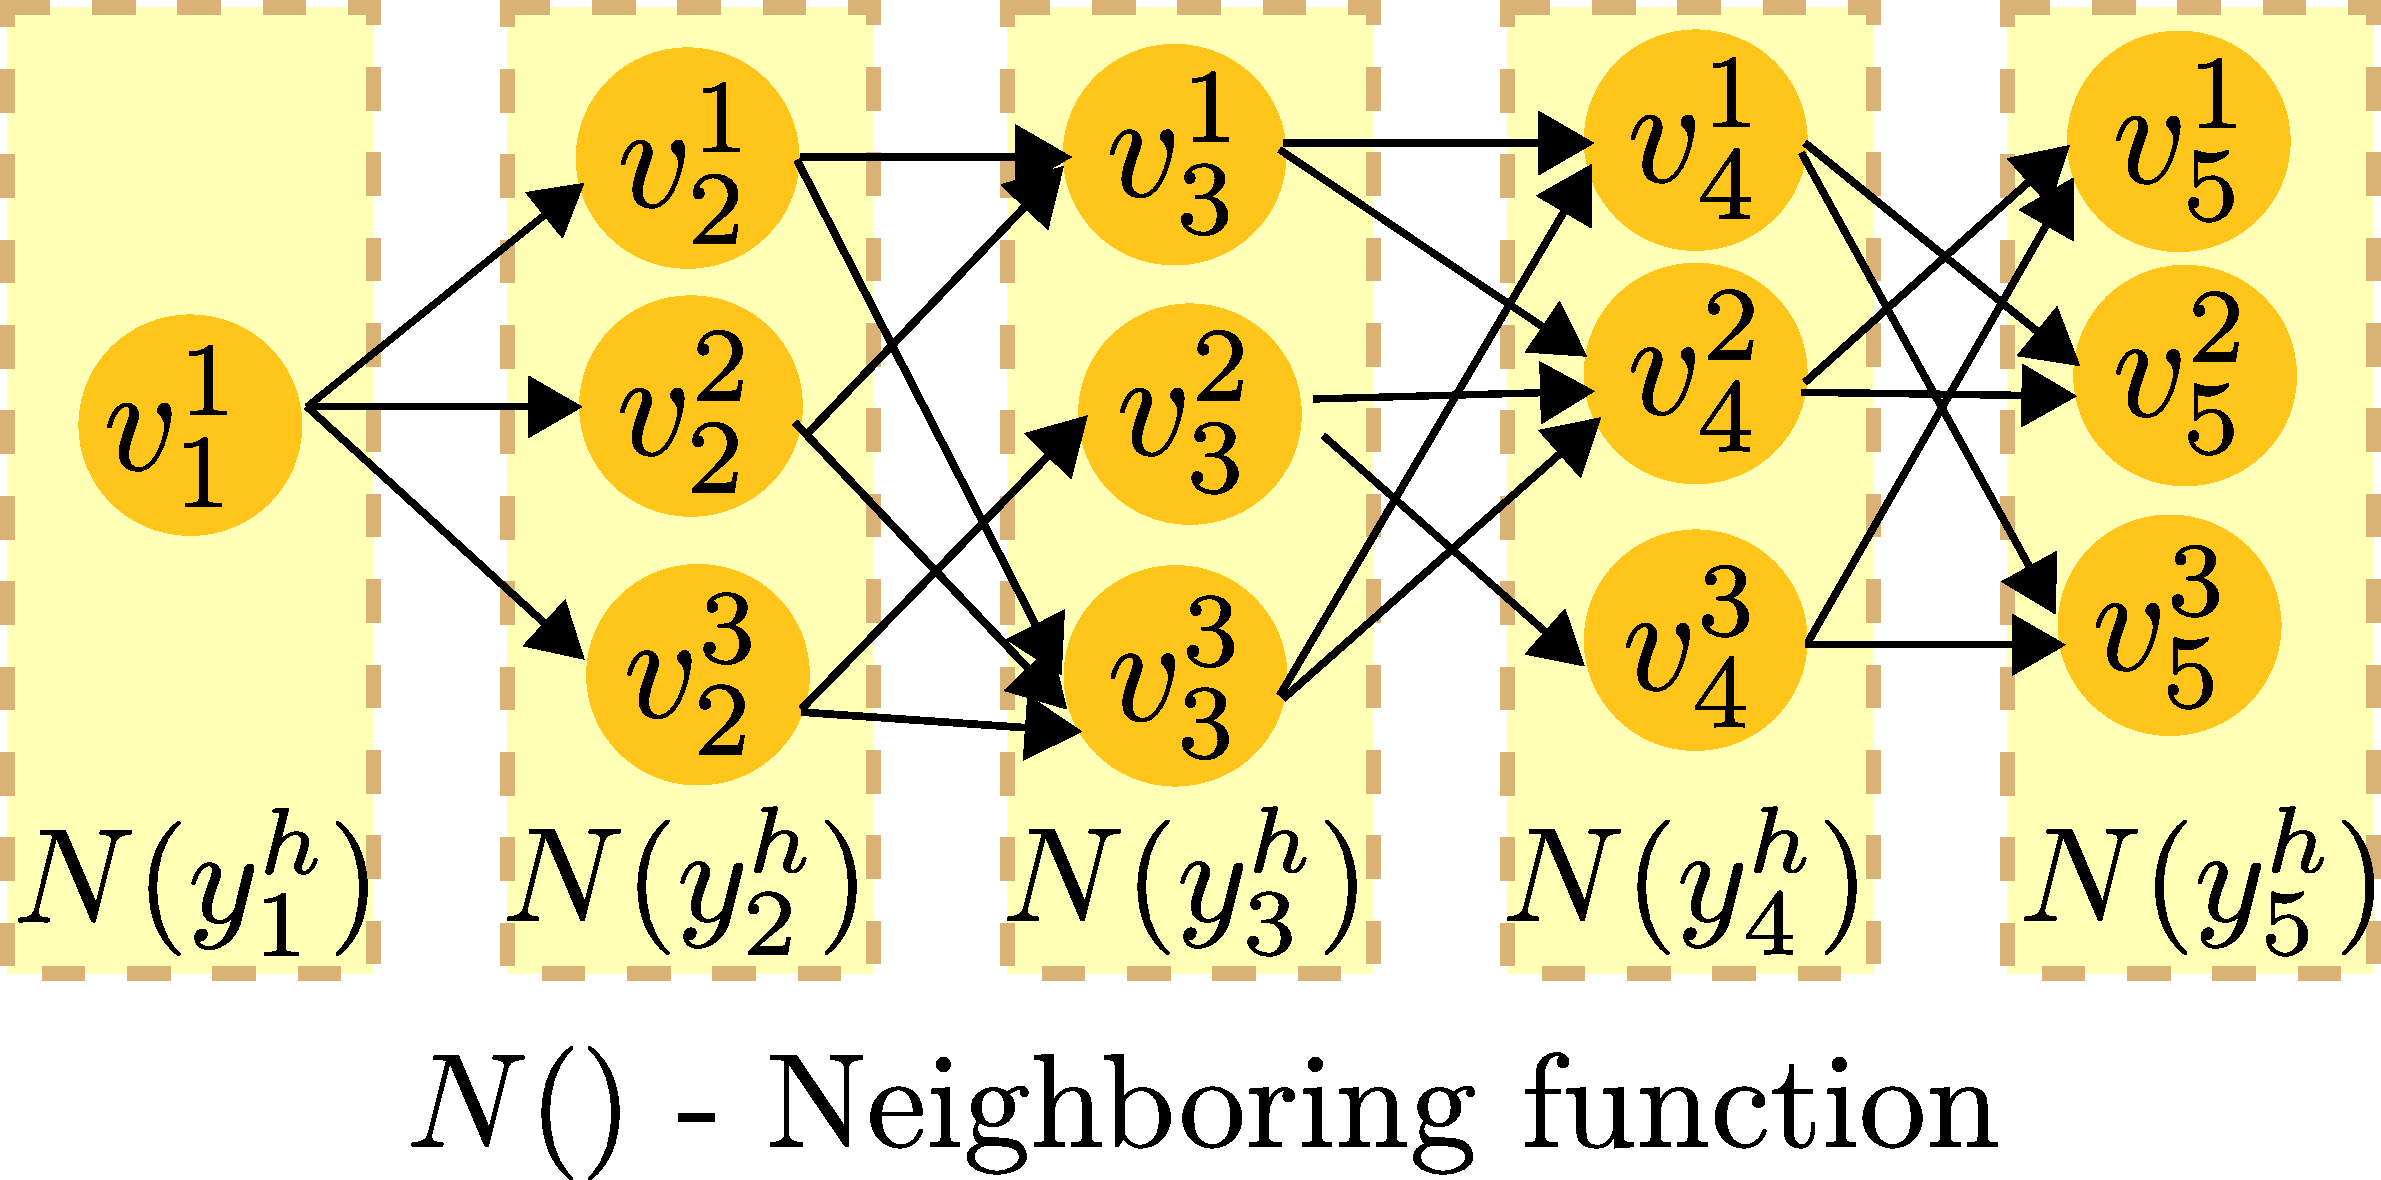
\includegraphics[width = 0.9\textwidth]{./figure/MultiPartite}
%\caption{A multi-partite graph generated from human constraint.}
\end{figure}
\end{minipage}

\column{.4\textwidth}
\begin{minipage}[c]{\linewidth}
%Multi-partite graph\\
%$ G = (V, E, T) $ 
%\begin{itemize}
%\item $ T $ - partition number
%\item $ V = \cup_{t=1}^{T} V(t) $
%\item $ (v^{i}_{t}, v^{j}_{t+1}) \in E $
%\end{itemize}
\end{minipage}

\end{columns}

\end{frame}

\begin{frame}{A pruning process}{The optimization model}

\begin{columns}

\column{.45\textwidth}

\begin{block}{Forward pruning}

Reachable

$ \forall t \in \{ 2, \cdots T \}, $ \\
$ \forall v \in V(t), deg^{-}(v) > 0 $

\begin{figure}
\centering
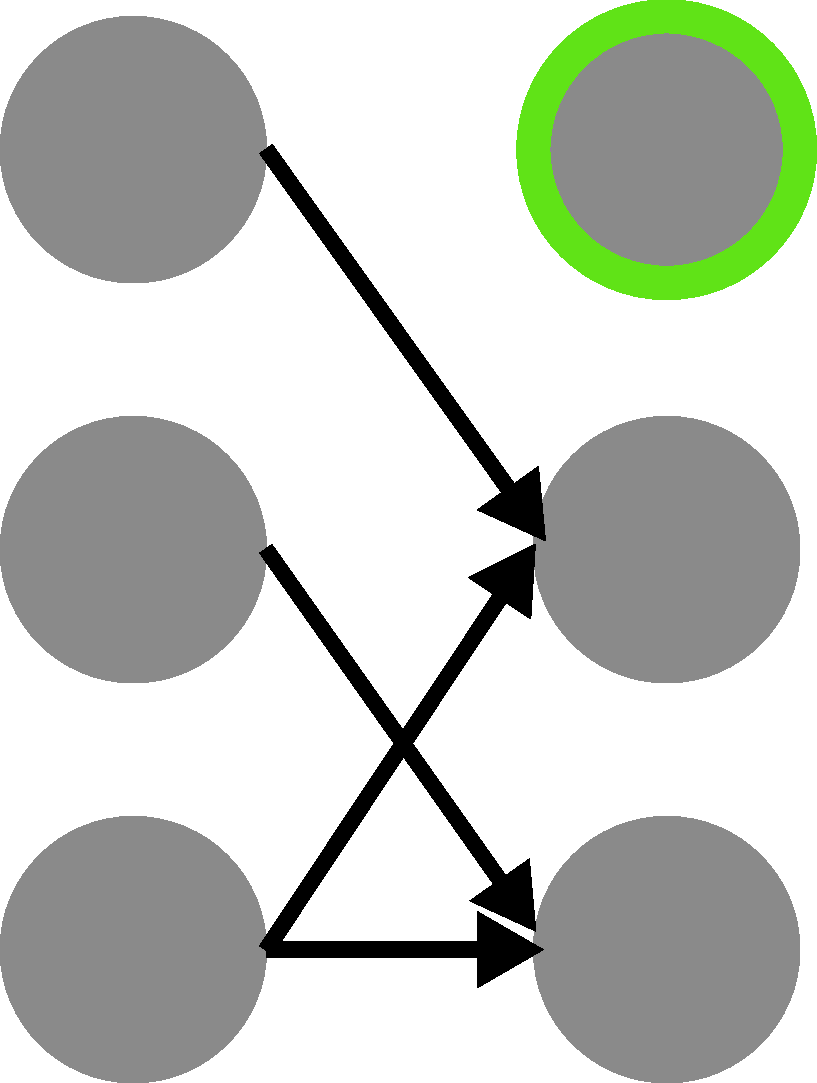
\includegraphics[width = 0.4\textwidth]{./figure/forward_prune}
\end{figure}

\end{block}

\column{.45\textwidth}

\begin{block}{Backward pruning}

Non-terminating 

$ \forall t \in \{ 1, \cdots T-1 \}, $ \\
$ \forall v \in V(t), deg^{+}(v) > 0 $


\begin{figure}
\centering
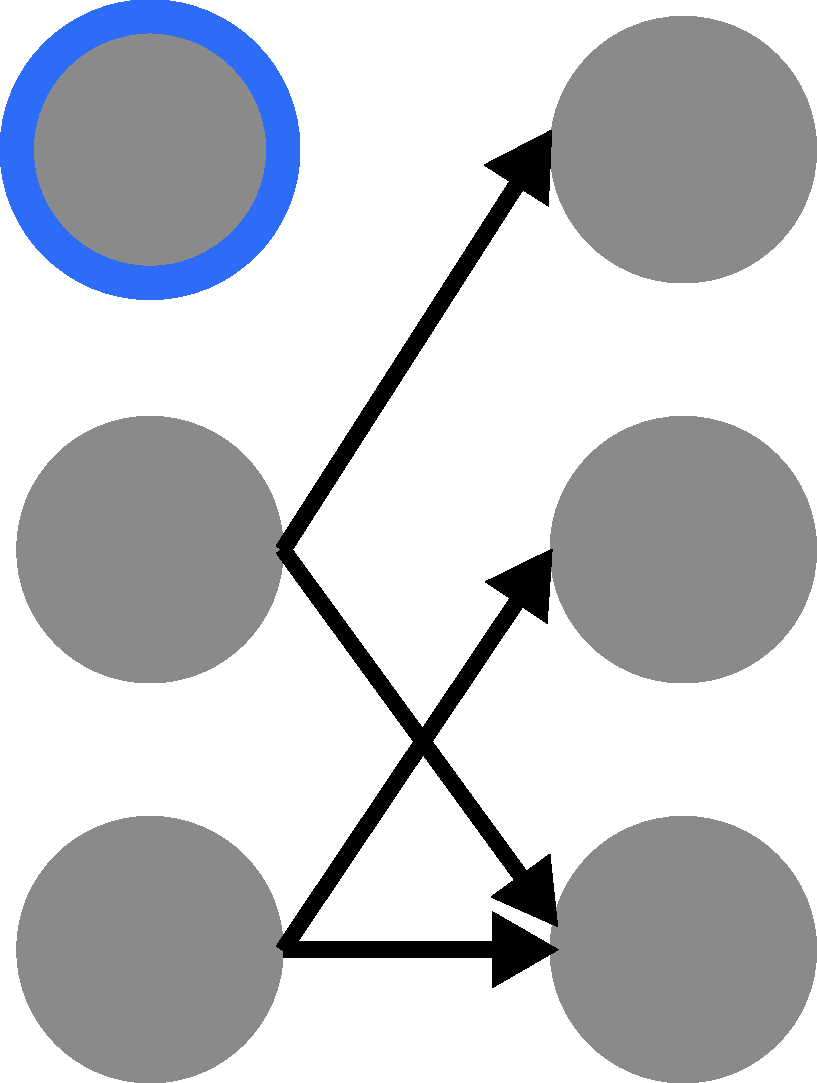
\includegraphics[width = 0.4\textwidth]{./figure/backward_prune}
\end{figure}

\end{block}

\end{columns}

\end{frame}

\begin{frame}{Obstacles}{The optimization model}

\begin{figure}
\centering
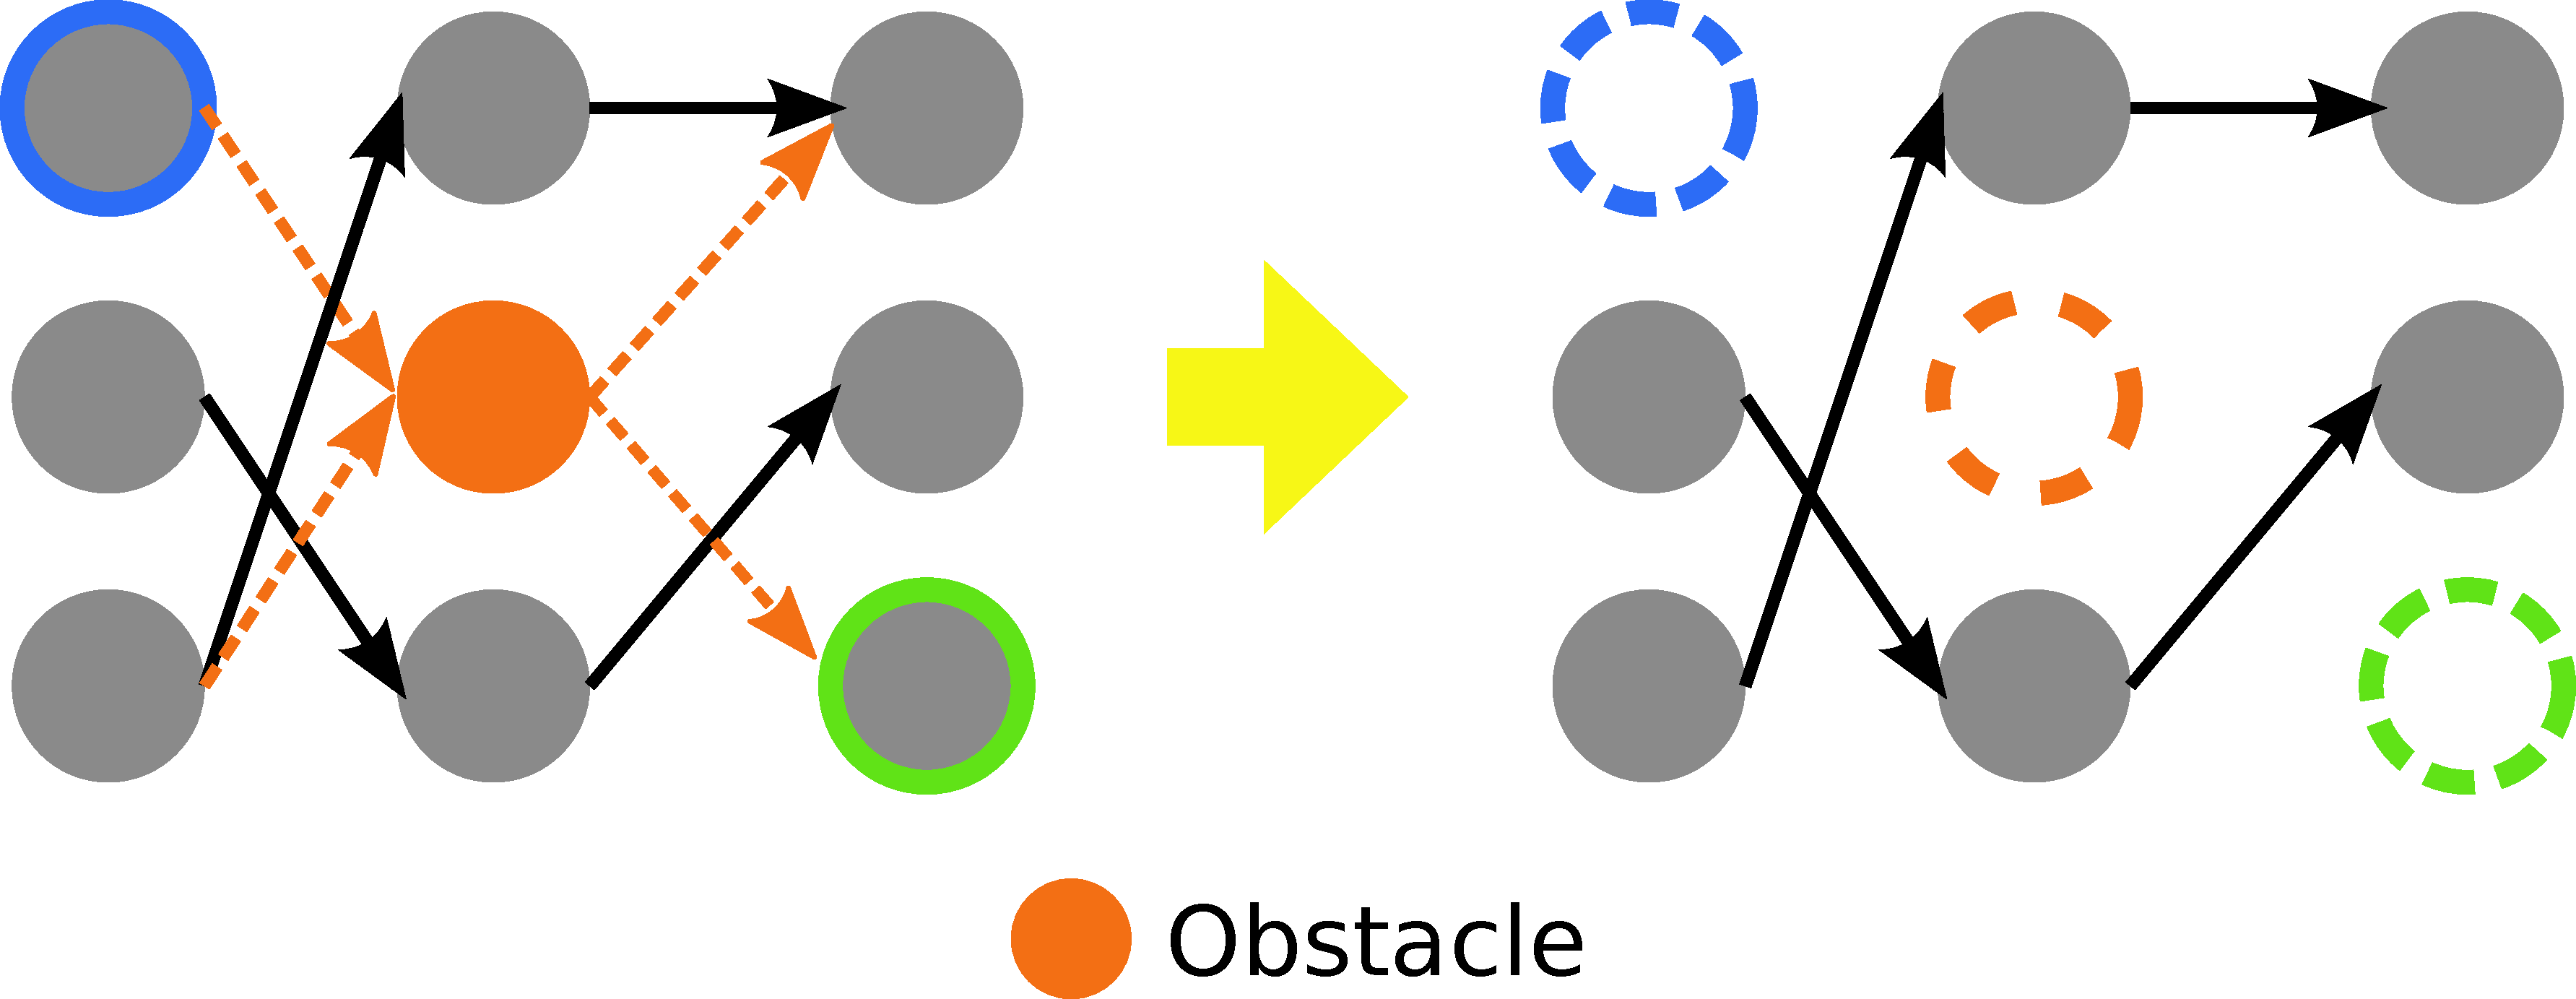
\includegraphics[width = 0.8\textwidth]{./figure/obstacle}
\end{figure}

\end{frame}

\begin{frame}{Submodular orienteering on a multi-partite graph}{The optimization problem}

\begin{equation}
\nonumber
\begin{aligned}
Objective: & X^{*} = \argmax_{X} \: f(X); \\
Constraint: & |X| = T, x_{t} \in V(t), (x_{t}, x_{t+1}) \in E.
\end{aligned}
\end{equation}

\end{frame}

